\documentclass[12pt, a4paper]{scrreprt}

\renewcommand*\familydefault{\sfdefault} 
%\usepackage[T1]{fontenc}

\usepackage[ngerman]{babel}
\usepackage{cite}
\usepackage[utf8]{inputenc}
%\usepackage[onehalfspacing]{setspace}
\usepackage{geometry, textcomp}
\newgeometry{right=2cm,left=4cm, top=2.5cm, bottom=2.3cm, footnotesep=0.5cm}

\usepackage[acronym]{glossaries}	% creates a glossary
\glsenablehyper
\makeglossaries

\usepackage[automark,headsepline,ilines,komastyle]{scrpage2}
\usepackage{amsmath,amssymb,amstext}
\usepackage{blindtext}
\setlength{\parindent}{0pt}
\setlength{\headheight}{1.5\baselineskip}
\renewcommand{\baselinestretch}{1.5}

\pagestyle{scrheadings}
\clearscrheadfoot
\ihead[]{}
\chead[]{}
\ohead[]{\headmark \hfill \thepage}
\ifoot[]{}
\cfoot[]{}
\ofoot[]{}

\setheadsepline[\textwidth]{1pt}
\usepackage{tabularx}
\usepackage{colortbl}
\usepackage{multirow}
\usepackage{hhline}
\usepackage{array}
\usepackage{tocloft}
\usepackage[hidelinks]{hyperref}
\tocloftpagestyle{scrheadings}
\renewcommand{\chapterpagestyle}{scrheadings}
\usepackage[font=footnotesize]{caption}

\usepackage{tikz}
\usepackage{rotating} 

\newenvironment{packed_item}
	{\begin{itemize}
			\setlength{\itemsep}{0pt}
			\setlength{\topsep}{0pt}
			\setlength{\parsep}{0pt}
			\setlength{\parskip}{0pt}}
		{\end{itemize}}
	
\usepackage[style=authoryear, natbib=true, backend=biber]{biblatex}

\renewcommand{\nameyeardelim}{ }
\usepackage[babel,german=guillemets]{csquotes}

\makeatletter

\newrobustcmd*{\parentexttrack}[1]{%
	\begingroup
	\blx@blxinit
	\blx@setsfcodes
	\blx@bibopenparen#1\blx@bibcloseparen
	\endgroup}

\AtEveryCite{%
	\let\parentext=\parentexttrack%
	\let\bibopenparen=\bibopenbracket%
	\let\bibcloseparen=\bibclosebracket}

\makeatother

\usepackage{pstricks}
\usepackage{pstricks-add}


\addbibresource{Lit.bib}
\usepackage[final]{pdfpages}

\newacronym{tmg}{TMG}{Telemediengesetz}
\newacronym{bdsg}{BDSG}{Bundesdatenschutzgesetz}
\newacronym{uwg}{UWG}{Gesetz gegen unlauteren Wettbewerb}
\newacronym{seo}{SEO}{Search Engine Optimization}






\begin{document}
		\begin{titlepage}
			\begin{center}
				\begin{spacing}{2}
					\includepdf{Image/FOM_Logo.pdf}
					\textbf{\large FOM - Hochschule für Oekonomie \& Management \\
						Hamburg \\
						\ \\
						Master-Studiengang Big Data \& Business Analytics \\
						x. Semester \\
						\ \\
						Titel\\
						Titel\\
						Titel 
						}
				\end{spacing}

				\vfill
				
				\begin{tabbing}
					\hspace{2.5cm}\=\kill
					Betreuer: \>  \\
					\> Dozent im Fach \glqq \grqq \\
					\ \\
					Autor: \> Vorname Nachname \\
					\> Straße \\
					\> PLZ Ort \\
					\> Matrikel-Nr:  \\
					\> x. Fachsemester \\
					\ \\
					Ort, den \today
				\end{tabbing} 
			\end{center}
		\end{titlepage}

%\includepdf{Image/Deckblatt.pdf}

			\setcounter{tocdepth}{3}
			\setcounter{secnumdepth}{3}		
			\pagenumbering{Roman}
			\thispagestyle{empty}
			\pdfbookmark{\contentsname}{toc}\tableofcontents
			\newpage
			\listoffigures
			\listoftables
			\printglossary[type=acronym,style=listdotted,title=Abkürzungsverzeichnis,toctitle=Abkürzungsverzeichnis] 
			\newpage
			\pagenumbering{arabic}
			\thispagestyle{empty}

\chapter{Abstract}\label{abstract}
\ref{abstract}

\chapter{Introduction}\label{introduction}

\gls{lda} provides many advantages, such as that it is suitable for large data and that it performs very well in extracting topics for Indonesian text documents \footnote{\autocite{twinandilla_2018}}.

In the year 2000, more than 209,000 children and adults died of leukemia globally. This number keeps growing year by year \footnote{\autocite{tang}}.

This article is ordered as follows: section 1 \ref{related} will explore ...
section 2 \ref{lda} presents ... and section 3 \ref{all}. Section 4 \ref{development} focusses on the developed implementation and classification algorithm.

\chapter{Related work}\label{related}

In this section, some examples of using text mining techniques in biology or medicine are described.
Zhao et al.\footnote{\autocite{zhao_2016}} describe how topic modeling can be used to analyze \gls{ngs}. Generally, by implementing topic modelling, text corpus are generated.

In the beginning of every genome analysis, there are several important questions to ask. Jurca et al.\footnote{\autocite{jurca_2016}} recommend to ask the following questions: What are the top studied genes in breast cancer? What are the regulations and limitations of blood cancer research in every country? Which countries have studied the largest number of breast cancer? Which are the popular genes mentioned together by countries every year? Where do key genes lie in the soft clusters?

Jurca et al. describe a process to use large-scale text analysis of biomedical abstracts in order to generate new hypothesis about cancer biomarkers. The target is to develop a data mining methodology to find out the genes associated with cancer. By analyzing disease-specific gene expression, experimental data is being checked. The key question is whether a gene has indeed been upregulated or downregulated with respect to a disease.

According to Xu et al.\footnote{\autocite{xu_2013}}, \gls{mirna}s build a class of 17-27 nucleotides single-stranded \gls{rna} molecules that regulate gen expression post-transcriptionally. In the described text-mining process, Xu et al. identified nine \gls{mirna}s in bladder cancer and adopted protein-protein interaction sites between these miRNAs and target genes. The results of the analyzation process lead to two relationship types between bladder cancer and its \gls{mirna}: casual and unspecified. 

Topic modelling is not only used to analyze relationships between genomes but also to improve diagnoses for stroke disease. Djatna et al. \footnote{\autocite{djatna_2018}} describe an 'Intuitionistic Fuzzy Based Decision Tree' to diagnose different types of stroke disease. To be precise, the different types of stroke diseases can be calculated by a Hamming distance. The term 'Fuzzy logic' means logic that underlies the reasoning of data using precise estimates. It is the fastest way to map input space into output space using a degree of membership.

Lloret et al.\footnote{\autocite{lloret_2012}} built an automatic summarization algorithm for literature. It can includes three steps: First, topic identification, second topic interpretation and third summary generation. While describing the process of textual analyzation, Lloret et al. mention a specific term: \gls{tf-idf} which is important for topic modelling. In addition to topic-based approaches, there are graph-based approaches and discourse-based approaches. Graph-based approaches implicate nodes that represent text elements and the edges/links refer to synonymy\footnote{\autocite{lloret_2012}}. Discourse-based approaches include \gls{rst}, \gls{hmm} or \gls{bm}. 

Yang et al.\footnote{\autocite{yang_2018}} describe the process of 'constructing a database for relations between human \gls{cnv}s and human genetic disease via systematic text mining'. In general, \gls{cnv} can cause disease, e.g. by manipulating gene dosage, disruption, fusion or other genetic position effects. 
To be more precise, there can \gls{cnv} can lead to two types of autosomal variants: They can either cause deletion or amplification of the long or broken arm region of chromosomes 1-22 or can build multiples of chromosomes 1-21 (e.g. as in disease trisomy 21). 

According to their article, Yang et al.\footnote{\autocite{yang_2018}} used a \gls{cnv} database which linked the \gls{cnv} information to the \gls{ncbi} Gene and Ontology database. Yang et al. mention three steps in the text mining process. First, during the pre-processing step, unstructured fields are split into separated sentences by using \gls{nltk}, a python package\footnote{\autocite{nltk}}. After that, in the \gls{ner} step, all disease mentions within the DNorm system, such as MeSH IDs are recognized. In the third step, \gls{re}, the positions in sentences and entities are compared to generate instances that constist of two candidate entities within one single sentence.
Yang et al. mention two more processing methods: Parallel Processing and Post Processing which includes data cleaning and statistics. The term 'data cleaning' is explained as 'de-duplicating data after each step of the process to reduce repetitive operations and prevent statistical errors'. This is a very useful step in biomedicine since biomedical databases may contain errors. For that reason, users can give feedback through a feedback mechanism to improve the quality of the databases.

Lu et al.\footnote{\autocite{lu_2016}} used multi-channel \gls{lda} to model healthcare data. In fact, by creating a learned latent variable model, the likelihood of a set of diagnosis, medications, contextual information in a patient's record can be evaluated. This can help to identify outliers and improve medical data quality. Furthermore, disease groups can be identified,  or missing medication or diagnosis can be predicted. Lu et al. used \gls{arm} and supervised learning to predict missing medications. The topic model defines how words in a document are generated through the control of latent topics.

\chapter{\gls{lda}}\label{lda}
\section{General description}\label{lda_description}
\gls{lda} was developed by David Blei et. al in the year 2003 and is a clustering algorithm for text mining. It counts to the most popular topic modelling algorithms\footnote{\autocite{zhao_2016}}.
According to Zhao et al., topic modelling requires of a number documents which represent each of them a mixture of latent topics. Moreover, each topic is expressed by a distribution of words. During \gls{lda}, two relationships are analyzed: First, the relationship between documents and words, also called 'per-document topic distributions'. Second, the relationship between words and topics ('per-topic word distributions'). To measure the relationships exactly and to make inference about topics and documents for text mining, probability matrices are calculated.

Park et al.\footnote{\autocite{park_2009}} define topic models as follows: Documents are no longer a collection of words, but a collection of topics. Furthermore, \gls{lda} is a generative topic model which uses a dirichlet parameter (also called dirichlet prior) to model documents. By changing the dirichlet prior, the number of topics that the model assigns to each word and document can be controlled. To be more precisely, a small dirichlet prior means a small number of topics assigned to each word. By increasing the dirichlet prior, the distribution of topics to each word rises. Moreover, the dirichlet parameter is obtained for each document and can be fitted using a maximum or estimated likelihood. If the dirichlet parameter does not fit, the gain in computational efficiency is obtained. Otherwise, there is no advantage (when dirichlet parameter fits well).

According to Jurca et al.\footnote{\autocite{jurca_2016}} the text mining process can be divided into four steps: First, the information has to be retrieved by user queries (\gls{ir}). Second, different vocabularies and ontologies have to be integrated (\gls{ner}). Third, during \gls{ie}, relationships between biological entities in the texts are extracted by either using co-occurence processing or \gls{nlp}. Last, there has to be gained biologically meaningful knowledge about how biological entities are related by implementing \gls{kd} methods.
Moreover, there can be distinguished between three types of clustering: hard clustering, hierarchical clustering and soft clusternig. Hard clustering describes the process of separating items into distinct groups where each item is exactly in one cluster. Hierarchical clustering implicates creating single-link clusters (how similar the items are to one another) and complete-link (how dissimilar the items are). Soft clustering means that items cannot be distinctly separated into clusters and partly are member of two or more clusters at a time.  

Besides, Djatna et al.\footnote{\autocite{djatna_2018}} mention data mining techniques, such as \gls{cart}, \gls{id3}, \gls{dt}, \gls{pca} and \gls{lda}. 

Lu et al.\footnote{\autocite{lu_2016}} define topic models as a text mining approach that assumes observed word co-occurences which are governed by latent variables. \gls{lda} includes the identification of latent topics from a set of documents, analyzing long-term topic trends and modelling words and references in documents.   

According to Hoffman et al., \gls{lda} is a probabilistic (Bayesian) model of text documents\footnote{\autocite{hoffman_2010}}. The idea of \gls{lda} is to define a document as a collection of k topics. Each topic defines a multinominal distribution over a vocabulary which is drawn from a dirichlet.

What is more, every term has a probabilistic relationship to every document. The topic model probabilities are stored as term relationships in thesaurus. The term frequencies are stored in the document index.

Twinandilla et al.\footnote{\autocite{twinandilla_2018}} mention three variables to be defined before the \gls{lda} process: $\alpha$ (the diversity of sentence distribution), $\beta$ (the diversity of topic distribution) and $\gamma$ (the similarity between sentences and titles).

In their article 'Multi-document summarization using k-means and \gls{lda}-significant sentences, Twinandilla et al. \footnote{\autocite{twinandilla_2018}} describe the research process by implementing the following six steps.

\begin{description}
\item[1.Step: Preprocessing]\hfill \\
First, all words and sentences need to be simplified by using a bag of words as well a bag of sentences. In detail, this step includes case folding (putting all words into lower case), tokenization (cutting a document into an array of words or sentences and eleminating punctuation), stopword removal (deleting words that appear often without a particular meaning) and stemming (changing words in a document that appear often wothout a particular meaning).

\item[2.Step: Calculate the number of clusters]\hfill \\
Second, the number of clusters needs to be calculated by using k-means clustering. 

\item[3.Step: \gls{lda}]\hfill \\
In this step, Twinandilla et al. distinguish between generative and inference \gls{lda}. Generative \gls{lda} forms a document from a collection of words whereas inference \gls{lda} only retrieves information from documents.

\item[4.Step: Sentence \gls{lda}]\hfill \\
Fourth, during sentence \gls{lda}, documents are represented as topic representation. Each topic is a sentence distribution that represents a sentence. This sentence has significant weight on a multi-document summarization.

\item[5.Step: Summary formation]\hfill \\
In this step, each document is sorted by a decreasing value of the final sentence weight. After that, the p percent of sentences with the highest value has to be chosen from each document. The p value is subsequently called 'summarization level'.

\item[6.Step: Arrange selected sentences in a sequence]\hfill \\
The last step includes the arrangement of all selected sentences in a sequence. This means putting them into a useful order to summarize all documents.
\end{description}

As reported by Blei et al.\footnote{\autocite{blei_2003}}, \gls{lda} is a generative probabilistic model for collections of discrete data such as text corpora. In addition to that, \gls{lda} is represented as three level hierarchical Bayesian model in which each item of a collection is a finite mixture over an underlying set of topics. What is more, each topic is modeled as an infinite mixture over an underlying set of probabilities. Blei et al. define topic probabilities as an explicit representation of a document.

\paragraph{\gls{tf-idf}}

\gls{tf-idf} is a scheme through which a basic vocabulary of words or terms is chosen. For each document in the corpus a count (which represents the number of occurences for each word) is formed\footnote{\autocite{blei_2003}}. 
There are three terms to be distinguished: First, a word is a basic unit of descrete data, defined to be an item from the vocabulary indexed by {1...V}. Second, a document is a sequence of N words. Third, a corpus is a collection of M documents.
After a suitable normalization process, the term frequency count is compared to an inverse document frequency count. This leads to the total number of occurences of a word in the entire corpus.
The result is a term-by-document matrix X whose columns contain \gls{tf-idf} values for each document in the corpus. 

\paragraph{\gls{lda} process}

The process of \gls{lda} can be briefly described with the following step\footnote{\autocite{wang_2008}}: First, there are M documents in the corpus. Second, each document j has \(N_{j}\) words. In the next step, the observed value \(w_{ji}\) describes the appearance of a word i in a document j. In addition to that, all words will be clustered into K topics which are defined as object classes. Finally, each topic k is modelled as a multinomial distribution over the codebook.

As reported by Wang et al., \gls{lda} is a language model which clusters co-occuring words into topics. Moreover, documents are described as 'bag of words'. 
Wang et al. describe a special form of \gls{lda}: Spatial \gls{lda}. It encodes spatial structure among visual words, assuming the partition of words into documents is known a priori. 

\paragraph{\gls{lda} extensions}

Extensions of \gls{lda} are author-topic model, dynamic-topic model and correlated topic model. Wang et al. refer to the dynamic-topic model while describing how visual words are clustered into topics which correspond to object classes.
 
\section{Examples and possible use cases}\label{lda_examples}

Zhao et al. describe the process of analyzing genomes as follows: First, each document corresponds to one of the total number of \gls{dna} straints. Second, all documents had the same number of words. Third, the distribution of words for topics as well as the distribution of topics in documents were described by random variables obeying Dirichlet distributions with parameters $\alpha$ and $\beta$. After that, nucleotides and their orders in \gls{ngs} sequences could be treated as words and the genetic information in sequences was translated and exhibited as a 'bag of words'\footnote{\autocite{zhao_2016}}. By using the strain-topic matrix derived from topic modelling, relationships or similarities between the strains serotypes can be found out. 

Hoffman et al.\footnote{\autocite{hoffman_2010}} describe the development of an online variational Bayes algorithm for \gls{lda} which is based on stochastic optimization with a natural gradient step. This step converges to a local optimum of the variational Bayes objective function.
To be more precise, Bayesian models provide a natural way to encode assumptions about observed data.
There can be distinguished between two approaches: First, sampling approaches are based on \gls{mcmc} sampling. Here, a Markov chain defines the stationary distribution.
Second, there are optimization approaches which are usually based on variational inference \gls{mcmc}. In this case, variational Bayes optimizes the simplified parametric distribution.

Twinandilla et al.\footnote{\autocite{twinandilla_2018}} developed a 'multi-document summarization using k-means and \gls{lda}-significant sentences' on yellow journalism. The term 'yellow journalism' stands for 'redundant news documents' which makes it difficult to distinguish documents containing fact or opinionated information. After defining the corpus, Twinandilla et al. describe two different summarization processes: Abstractive as well as extractive summarization. Abstractive summarization means summarizing documents by creating new sentences (with the same information as the original document). Extractive summarization suggests summarizing a document by selecting a part of a sentence in that document.

As described in chapter \ref{related} on page \pageref{related}, Lu et al.\footnote{\autocite{lu_2016}} used \gls{mclda} to estimate latent health status groups. \gls{mclda} constructs latent relations among diagnoses, medications, contextual variables in different status groups. To be more precise, it is a dimensional reduction method that summarizes each record using a probability vector over a latent health status group. The prediction tasks were performed by using a \gls{cgs} based inference model and inferred methods. 
During the topic modelling process, Lu et al. refer to two associations among the data: diagnosis-medication associations to identify the clinical use of medications and diagnosis-diagnosis associations to create a network structure among the diseases.

Lee et al.\footnote{\autocite{lee}} analyzed the direct and indirect interactions between \gls{dna} copy number and gene expression changes. 'DNA copy number aberrations and gene expression changes provide valuable information for studying chromosomal instability and its consequences in cancer.' Three types of cancer have been analyzed: brain, bladder and breast cancer. The results of the analysis lead to a significant association between \gls{dna} copy number and its gene expresion. By monitoring gene expression data, different classes of tumors can be distinguished successfully.
  
\section{Python library 'Gensim'}\label{gensim}
'Gensim' stands for 'generate similar' and is a python library, created by Radim Rehurek and Petr Sojka \footnote{\autocite{gensim}}. Firstly created in  2008, it was a collection of various Python scripts to generate a short list of the most similar articles to a given article. Gensim supports scalable statistical semantics to analyze plain-text documents for semantic structure and to retrieve semantically, similar documents.            
              
\chapter{Acute Lymphoblastic Leukemia}\label{all}
\section{Types of Leukemia and its causes}\label{leukemia_types}
According to Jurca et al.\footnote{\autocite{jurca_2016}}, cancer is the result of damage, especially of mutations to cell's \gls{dna} which leads to a cell losing its normal functionality and gains the ability to indefinitely multiply until normal tissue funtions are impaired. This is also why malitious cancer is distributing so fast. Besides, each patient develops a different set of cancerous mutations in various genes which lead to multiple subtypes of cancer.
Furthermore, some genes can be up-regulated (which means that they are transcribed and expressed more), down-regulated (which means that they are not expressed) or can be co-expressed (which means that they are expressed at the same time).

As stated by Montano et al.\footnote{\autocite{montano_2018}}, \gls{all} is a malignant disorder originating from hematopoietic B-/T-cell precursors which are characterized by marked heterogenity at molecular and clinical levels. There are many approaches to analyze these precursors, such as analyzing targeting of transcriptional factors (PAX5) which are involved in the pathogenesis of B-ALL. Other therapeutic and clinical approaches are genome editing techniques, i.e. the design of new therapies (\gls{car}s) and the study of genes involved in the evolution of pathogenesis.

Jagadev et al.\footnote{\autocite{jagadev}} define leukemia as blood cancer which begins in the bone marrow where it causes formation of a large number of abnormal cells. According to Jagadev et al. there are four common types of leukemia: \gls{all}, \gls{aml}, \gls{cll}, \gls{cml}. Furthermore, the normal and leukemic lymphocytes differ significantly.

As explained by Tang et al.\footnote{\autocite{tang}}, every subtype of leukemia can have individualized treatments and therapies.

According to Andersson et al., \gls{all} is caused the expansion of immature hematopoietic cells (blasts) in the bone marrow and peripheral blood\footnote{\autocite{andersson}}. Furthermore, \gls{all} counts to the most common childhood malignancies, appearing between 2 to 5 years of age. \gls{all} has two subtypes: \gls{tall} and \gls{bcpall}.
The new cases of \gls{tall} are 15\% childhood and 25\% adult \gls{all}. Compared to \gls{bcpall}, \gls{tall} is characterized by older ages of onset, male sex predominance, inferior outcome and chromosomal abnormabilities.
In 1960, the 'Philadelphia chromosome' in \gls{cml} was discovered which groups it to 'genetic disease'.
The result of the exchange of genetic material between two chromosomes is called chromosomal translocations. These serve as hallmarks of leukemia and are intimately associated with a specific leukemia type and its prognosis. Moreover, the different types of \gls{all} are commonly associated with genetic events, such as \gls{cna}, a sub-microscopic deletions or gains,  amplifications and sequence mutations.

\paragraph{Therapies against \gls{all}}
The \gls{callcg} first met in 1994 to find out a specific treatment for childhood \gls{all}.
In 2009, \gls{callcg} describe a therapy using anthracyclines to treat childhood \gls{all}\footnote{\autocite{callcg_2009}}. In fact, some studies suggest that anthracyclines might cause cardiotoxicity. In most cases of the therapeutic approach, anthracyclines significantly reduced the bone marrow relapse when added to the standard therapy. But it did not significantly increase an event-free survival.
One year after that, \gls{callcg} reviewed the addition of vincristine plus steroid pulses (prednisone and prednisolone pulses) to the treatment of childhood \gls{all} \footnote{\autocite{callcg_2010}}. As a result, the combination of vincristine pulses significantly reduced the overall event rate by around 30\% to 10\% improvement in \gls{efs} by  five years.

\section{Examples for Genome Analysis: \gls{ngs}}\label{genome_analysis}
\gls{ngs} refers to post-Sanger sequencing methods\footnote{\autocite{zhao_2016}}. Since \gls{ngs} produces large volumes of sequence data it might be very useful implementing topic modelling techniques in order to maintain the flexibility for the level of resolution required for given experiments.  
According to Gasperskaja et al.\footnote{\autocite{gasperskaja_2017}}, \gls{ngs} does not require a priori knowledge about genomic feature, it only requires a low amount of \gls{dna} or \gls{rna} as input.

The step before analyzing two or more (multiple) genomes is called alignment which includes a comparison of two genomes. There are many different types of alignments, but Zhao et al. refer to the \gls{msa} by describing \gls{muscle} and CLUSTAL.

Gasperskaja et al. mention an important question which should be asked before every genome analysis: 'Is the variance pathogenic?' and whether there is any relationship between genotype and phenotype which means that it can lead to a disease or can cause a number of disorders. 
Moreover, there can be distinguished between beneficial (\gls{snp}) and pathogenic (nonsense variant) single nucleotide changes, large microscopically visible or chromosomal aberation. 
To find out whether a genome mutation is pathogenic, Gasperskaja et al. explain that substantial information about functional genomics can be found through the analysis of \gls{mrna} or \gls{crna} (which is a copy from \gls{mrna} by reverse transcription \gls{pcr}.
Methods to measure \gls{rna} expression are the following: \gls{sage} or \gls{qpcr}.
By using \gls{cdna} microarray assays important genome-wide information about changes of gene expression in various cell lines can be found out.

As claimed by Montano et al.\footnote{\autocite{montano_2018}}, the development of \gls{ngs} techniques implicates vast amount of data which need to be translated. One important question is to find out how the genotype (the genetic expression of a biological attribute) influences the phenotype. By integrating genome editing systems into their research process, investigators are able to manipulate virtually any gene in a diverse range of cell types and organisms.
To give an example, Gasperskaja et al. and Montano et al. describe \gls{crispr-cas9}. In fact, this genome analysis includes generating a direct cut in the double strand of \gls{dna} by Cas9 nuclease. Cas9 is driven by a single 20-nucleotide \gls{rna} strand which marks the direct breakpoint. After cutting the \gls{dna}, the repair machinery of the host cell repairs errors and promotes a modification of the original sequence by a mutation (e.g. insertion, deletion, inversion).
But why should be changed the shape of \gls{dna}? In the opinion of Montano et al.\footnote{\autocite{montano_2018}}, the use of genetically modified cell lines and animal models help us to better understand the functions of genes and their pathogenesis in diseases, such as cancer.
   
\section{Data sources: \gls{ncbi} and Ensembl genome browser 96}\label{datasources}

\paragraph{\gls{ncbi}}

\gls{ncbi} was established in Nov. 4, 1988 as a national resource for molecular biology information \footnote{\autocite{ncbi}}. Its main purpose was to create automated systems for storing and analyizing knowledge about molecular biology as well as biochemistry and genetics.The community of \gls{ncbi} conducts research on fundamental biomedical problems at a molecular level using mathematical and computational methods.
Moreover \gls{ncbi} collaborates with several \gls{nih} and develops, distributes, supports, and grands access to various databases and software for scientific and medical communities.
\gls{ncbi} also works as an organization for standardization of databases, data deposition and data exchange and biological nomenclature.
As a challenge, \gls{ncbi} needs to find new approaches to deal with the volume and complexity of data. Another complex issue \gls{ncbi} is facing is how to provide researchers better access to analysis and computing tools. These tools will be useful to understand the genetic legacy and its role in health and disease.

In this article, \gls{ncbi} was used to query all genomes related to the diseas \gls{all} which can be seen in figure \ref{ncbi_query}.
After selecting the first gene 'IKZF1', the web interface shows details about the given genome sequence (see figure \ref{gene_details}). Below the given point 'See related', a link to the related source from Ensembl genome browser 96 can be clicked. The next paragraph describes the information from the Ensembl genome browser 96.

% ncbi query for all genomes
\begin{figure}[htbp]
	\centering
	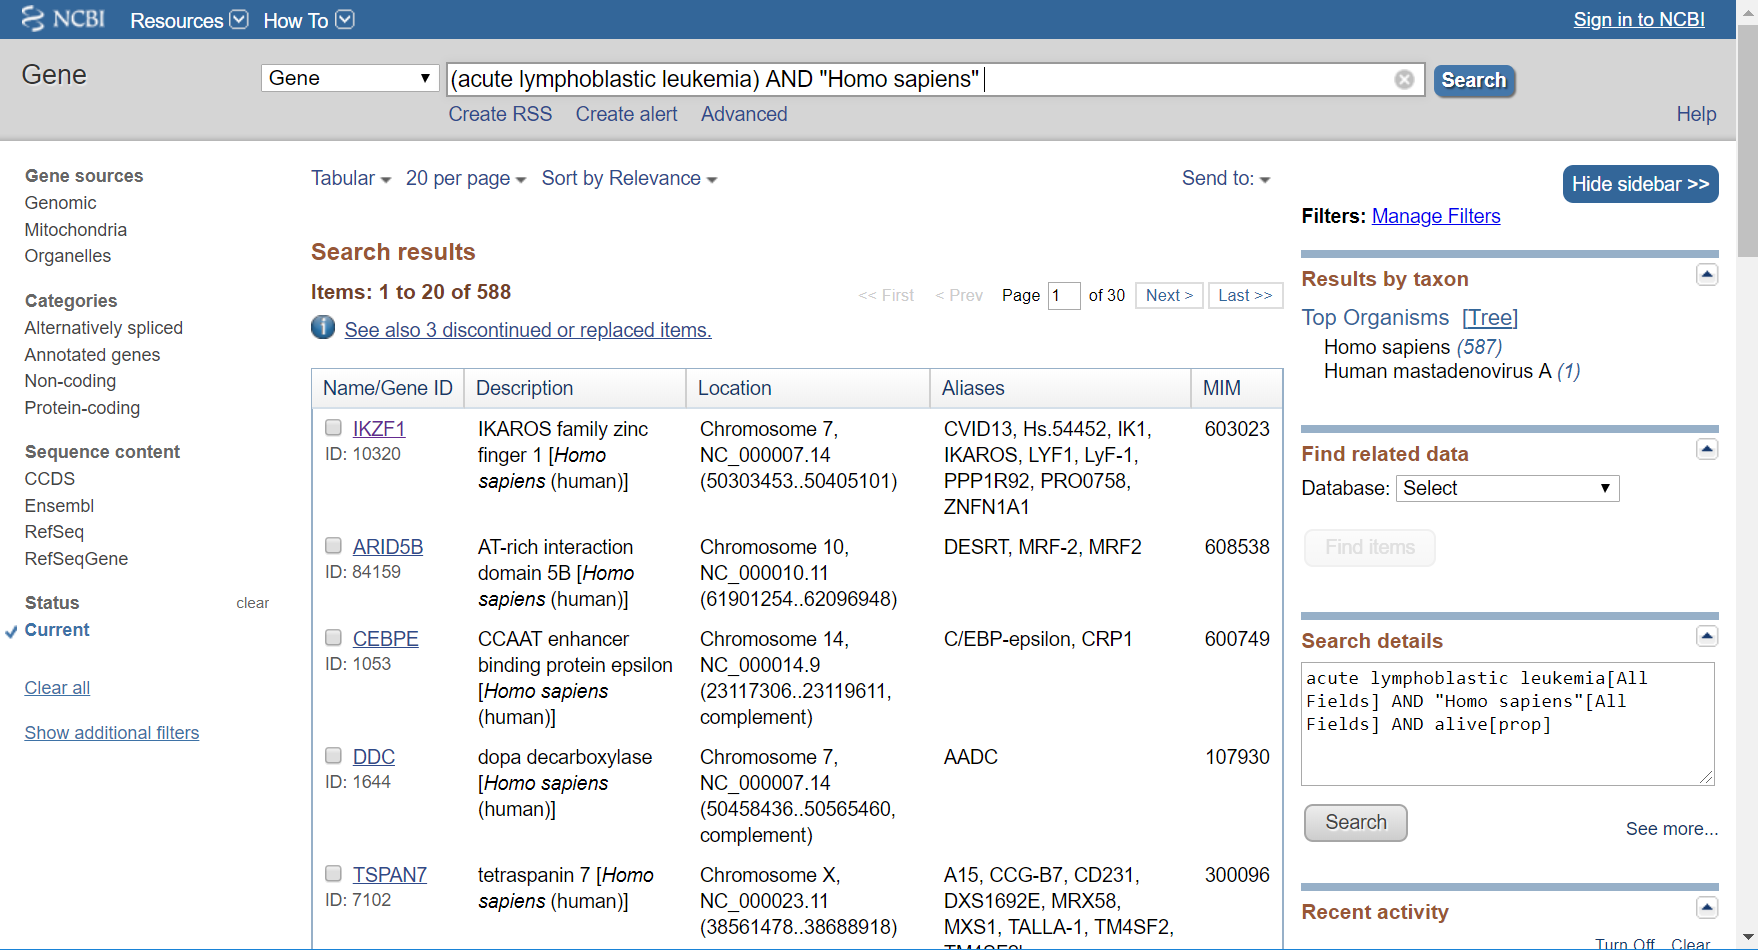
\includegraphics[width=1\textwidth]{Image/ncbi_all_result.png}
	\caption{\gls{ncbi} query to find all \gls{all} related gene sequences}
	\label{ncbi_query}
\end{figure}

% ncbi detail view for one genome
\begin{figure}[htbp]
	\centering
	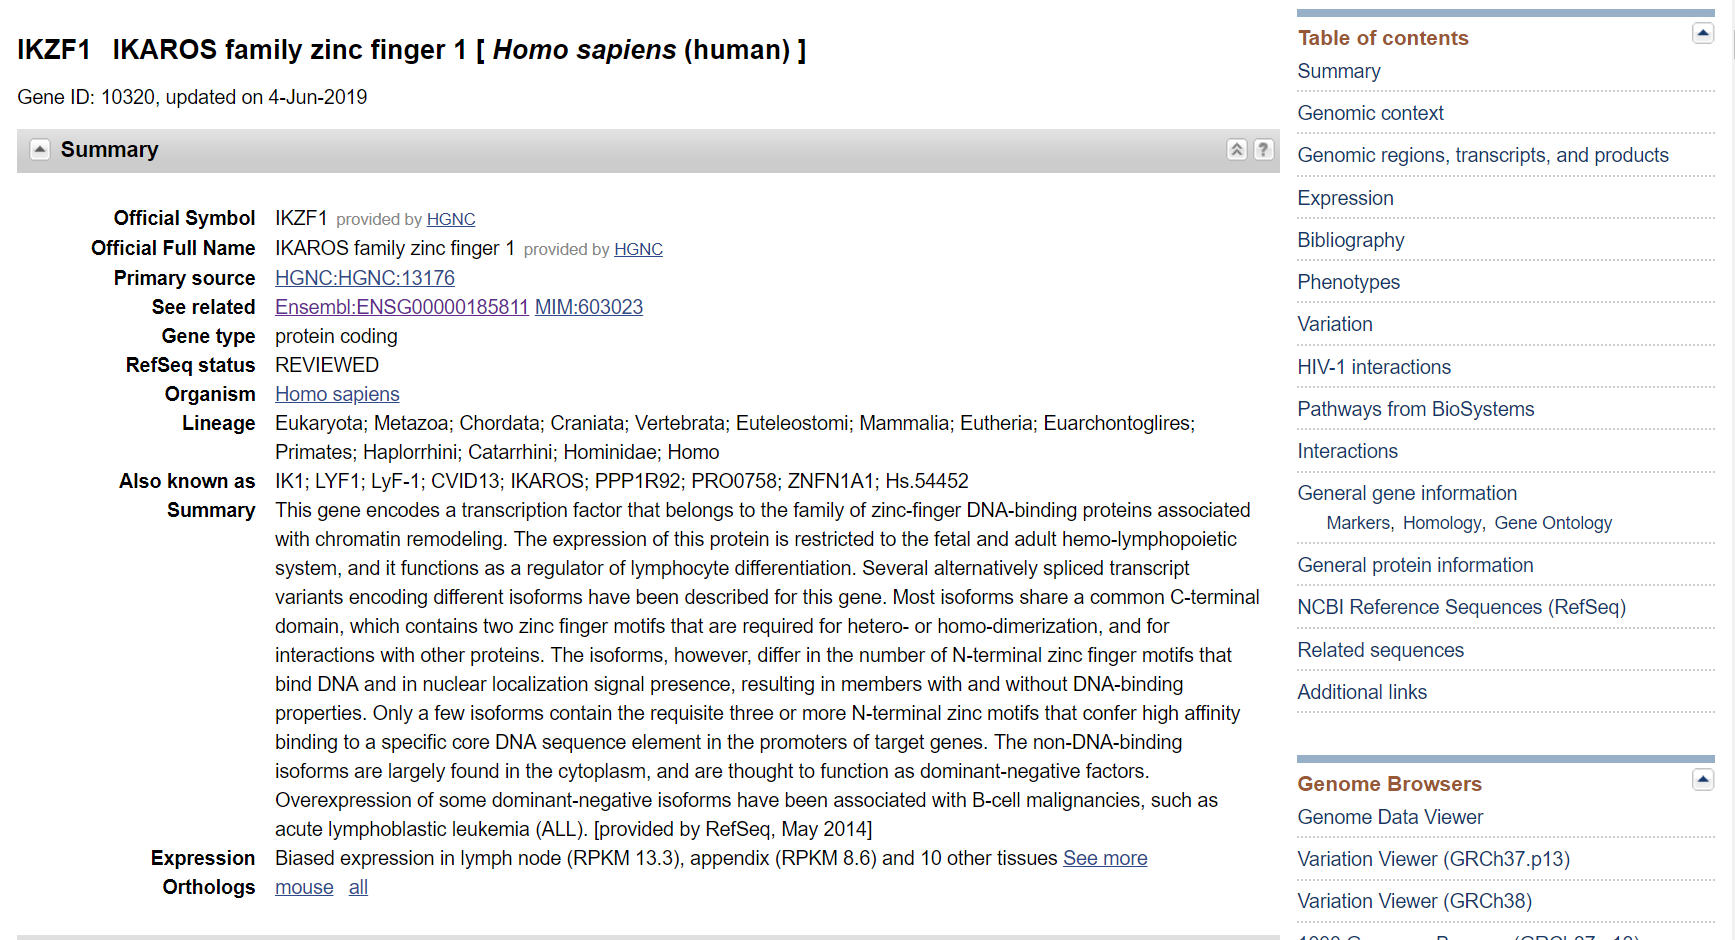
\includegraphics[width=1\textwidth]{Image/ncbi_gene_details.png}
	\caption{Detailed information about selected gene sequence}
	\label{gene_details}
\end{figure}

\paragraph{Ensembl genome browser 96}

The second genome database used in this article, was the Ensembl genome browser 96 \footnote{\autocite{ensembl}}. It is a special genome browser for vertebrate genomes. In comparison to \gls{ncbi}, Ensembl annotates genes and computes multiple alignments and predicts regulatory function. Besides, Ensembl collects disease data and supports research in comparative genomics, evolution, sequence variation and transcriptional regulation.
In April 2019, Ensembl published a new release which included a \gls{rest} and \gls{ftp} \gls{api}. Apart from new genomes, Ensembl Release 96 offers a new interface to configure the regulation tracks.

Figure \ref{ensembl_result} shows the Ensembl result of the selected gene from \gls{ncbi} database.

% ensembl result
\begin{figure}[htbp]
	\centering
	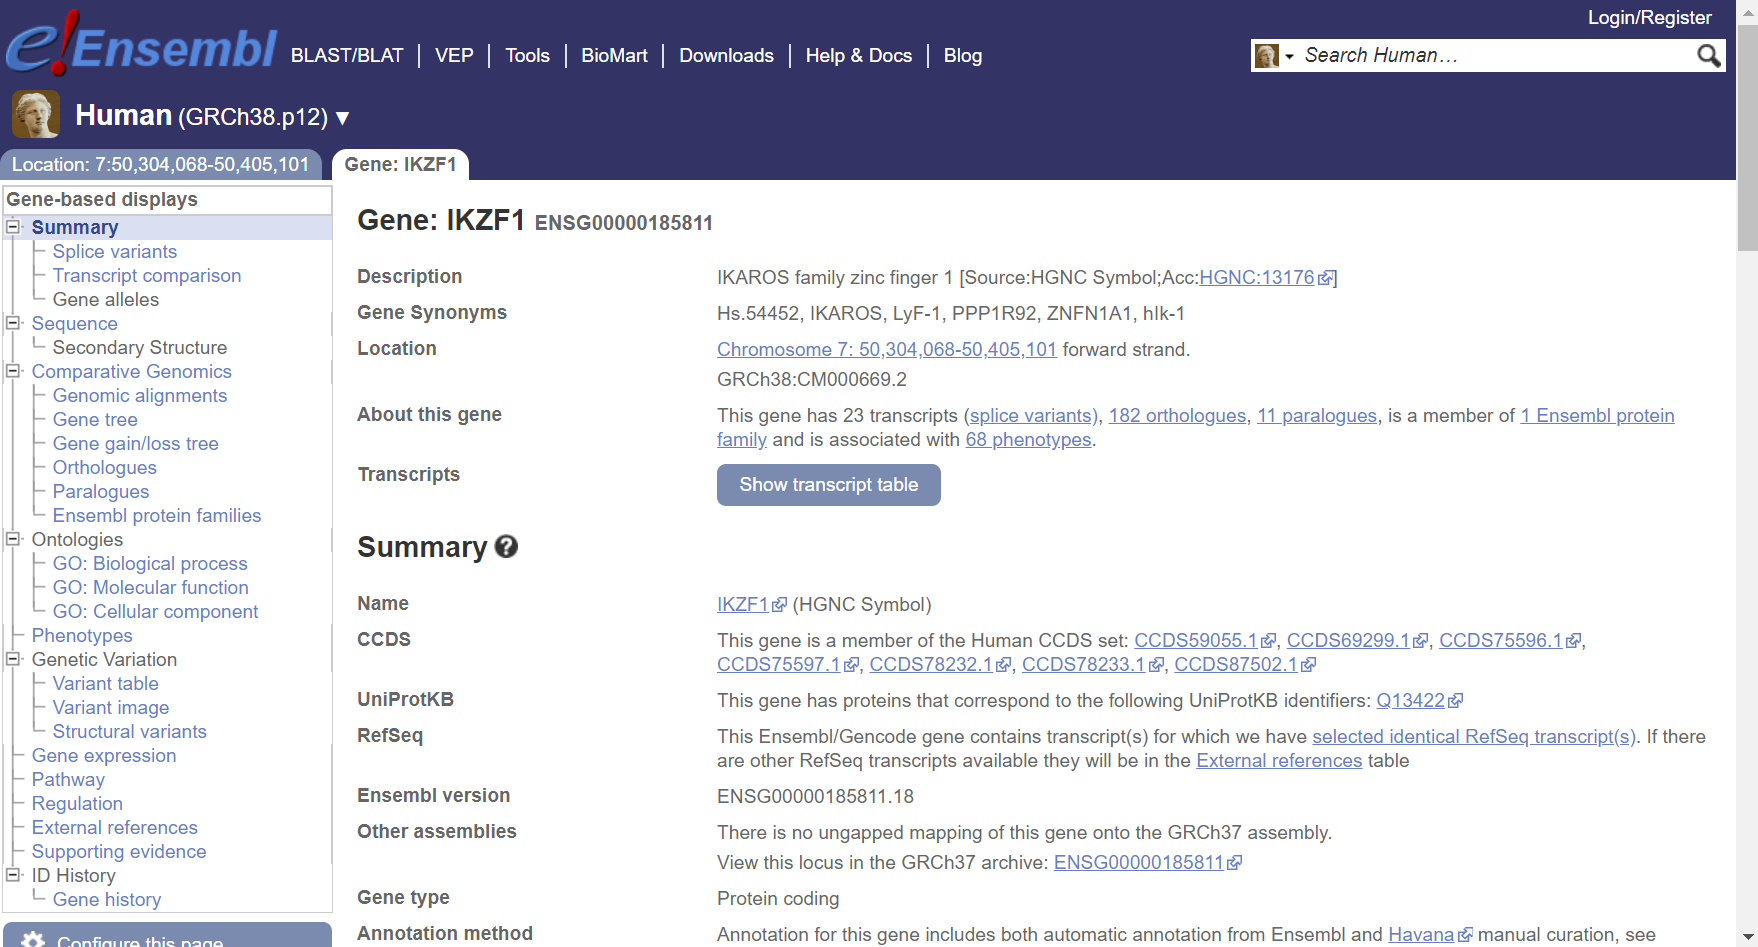
\includegraphics[width=1\textwidth]{Image/ensembl_ikzf1.png}
	\caption{Information about genome IKZF1, found in Ensembl genome browser 96}
	\label{ensembl_result}
\end{figure}

\chapter{Development of a solution for genetic analysis of \gls{all} genomes by implementing \gls{lda}}\label{development}
\section{Problems and challenges of genetic analysis}\label{problems_challenges}
Quality of data 
Is the data complete, which includes that it contains all required genomes which can cause \gls{all}.

our assumptions can lead to false content or solutions 

\section{First steps: Draft of developed solution}\label{draft}

To get useful data, the \gls{ncbi} \footnote{\autocite{ncbi}} was used to get all currently detected mutations of genomes which may cause \gls{lda}.

The first idea was to build a parsing application, which iterates over the found 582 genomes. After the iteration, it compares the oncogenes with the healthy genomes and to figure out where the differences are. The results might be displayed in a diagram. It might be possible to create clusters from the differences between the two groups or practice \gls{lda} on the differences.

\section{Proposed solution}\label{proposed_solution}

% algorithm to create topics
\begin{figure}[htbp]
	\centering
	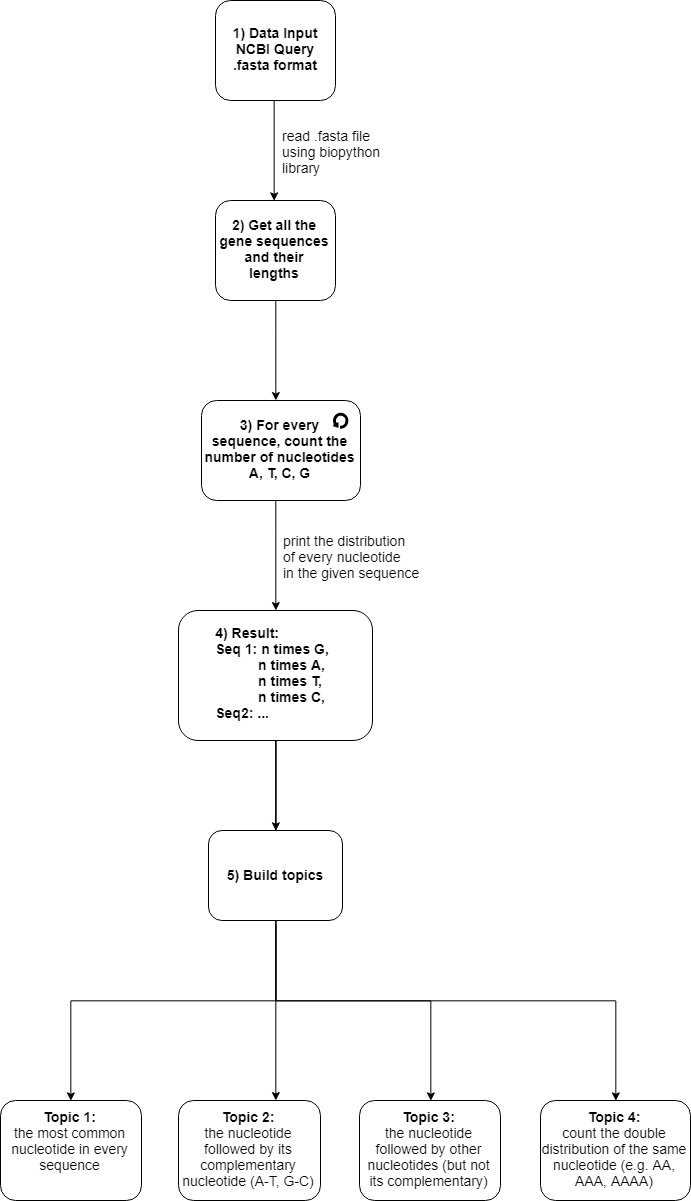
\includegraphics[width=1\textwidth]{Image/creating_topics_algorithm.png}
	\caption{Diagram of developed algorithm to create basic topics among given gene sequences}
	\label{algorithm_figure}
\end{figure}

\section{Results}\label{results}


\chapter{Conclusion and Outlook}\label{conclusion_outlook}
\section{Lessons learned}\label{lessons_learned}

There are many genome analysis tools in the internet. \gls{nih} provides several interfaces for genome alignment methods to find out the similarity between two given genome.\footnote{\autocite{blast}}.
But in the given case, all given gene sequences should be compared with each other in order to find appropriate clusters.


\section{Conclusion}\label{conclusion}
\section{Outlook}\label{outlook}	

\begingroup
	\setlength{\emergencystretch}{8em}
	\renewcommand{\bibname}{Literaturverzeichnis}
	\printbibliography
\endgroup
\newpage




\renewcommand{\bibname}{Rechtsquellenverzeichnis}

\makeatletter
\def\@biblabel#1{}
\makeatother


\begin{thebibliography}{0} 
%	\setlength{\leftmargin}{5cm}
	\setlength{\itemindent}{-0.2cm}
	\bibitem{} Bundesdatenschutzgesetz, BDSG, 1990, zuletzt geändert 2009
	\bibitem{} Gesetz gegen unlauteren Wettbewerb, UWG, 2004, zuletzt geändert 2013		
	\bibitem{} Richtlinie 95/46/EG des Europäischen Parlaments und des Rates vom 24. Oktober
	1995 NI. L 281/31 zum Schutz natürlicher Personen bei der Verarbeitung
	personenbezogener Daten und zum freien Datenverkehr
	\bibitem{} Telemediengesetz, TDG, 2007, zuletzt geändert 2010


\end{thebibliography}


\newacronym{tmg}{TMG}{Telemediengesetz}
\newacronym{bdsg}{BDSG}{Bundesdatenschutzgesetz}
\newacronym{uwg}{UWG}{Gesetz gegen unlauteren Wettbewerb}
\newacronym{seo}{SEO}{Search Engine Optimization}





\newpage

\ohead[]{Ehrenwörtliche Erklärung \hfill \thepage}

\null\vfill
\textbf{Ehrenwörtliche Erklärung}

Hiermit versichere ich, dass die vorliegende Arbeit von mir selbstständig und ohne unerlaubte Hilfe angefertigt worden ist, insbesondere dass ich alle Stellen, die wörtlich oder annähernd wörtlich aus Veröffentlichungen entnommen sind, durch Zitate als solche gekennzeichnet habe. Ich versichere auch, dass die von mir eingereichte schriftliche Version mit der digitalen Version übereinstimmt. Weiterhin erkläre ich, dass die Arbeit in gleicher oder ähnlicher Form noch keiner Prüfungsbehörde / Prüfungsstelle vorgelegen hat. Ich erkläre mich damit nicht einverstanden, dass die Arbeit der Öffentlichkeit zugänglich gemacht wird. Ich erkläre mich damit einverstanden, dass die Digitalversion dieser Arbeit zwecks Plagiatsprüfung auf die Server externer Anbieter hochgeladen werden darf. Die Plagiatsprüfung stellt keine Zurverfügungstellung für die Öffentlichkeit dar.

\ \\ \ \\ 


Ort, Datum (Vorname Nachname)

\vfill
\bibdata{Lit}



\end{document}
